\scanpage{154}
% position: top deleted tensor and decomposition
\deleted{\(E_1\otimes E_2\)}
\figure{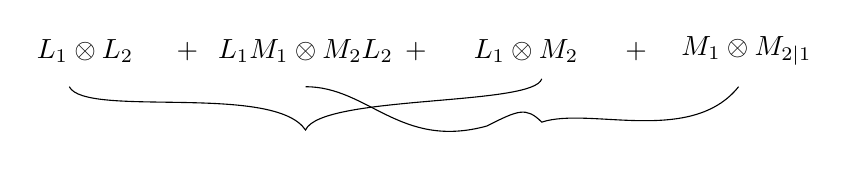
\begin{tikzpicture}[x=1cm,y=1cm]
\node at (0,0) {$L_1\otimes L_2$};
\node at (1.3,0) {$+$};
\node at (2.8,0) {$\unsure{\deleted{L_1}\inserted{M_1}}\otimes\unsure{\deleted{M_2}\inserted{L_2}}$};
\node at (4.2,0) {$+$};
\node at (5.6,0) {$L_1\otimes M_2$};
\node at (7.0,0) {$+$};
\node at (8.4,0) {$M_1\otimes M_{\unsure{2|1}}$};
\draw (-.2,-.45) .. controls (0,-.85) and (2.4,-.4) .. (2.8,-1.0)
 .. controls (3.0,-.55) and (5.7,-.7) .. (5.8,-.35);
\draw (2.8,-.45) .. controls (3.6,-.45) and (4.0,-1.25) .. (5.1,-.95)
 .. controls (5.5,-.75) and (5.6,-.7) .. (5.8,-.9)
 .. controls (6.4,-.7) and (7.7,-1.2) .. (8.3,-.45);
\end{tikzpicture}}
% position: upper diagram
\diagram{\begin{tikzcd}[column sep=large,row sep=large]
E_1\otimes_{0}E_2 \arrow[r,"F_{11}^{!}"] \arrow[dd] \arrow[dr,"\pi"'] \arrow[ddr,bend right=35,dash]
 & E_1\otimes E_2 \arrow[r] & E_1\otimes^{0}E_2 \\
 & L_1\otimes\unsure{L_2|E_2} \arrow[u,"\alpha_1\otimes\alpha_2"'] \arrow[ur,bend right=15,dash,"\deleted{\uline{\unsure{comm.}}}"'] & \\
E_1\otimes\unsure{E_2|\Omega} & M_1\otimes M_2 \arrow[l,"\psi_1\otimes\psi_2"] \arrow[uur] &
\end{tikzcd}}
% reading question: the lower horizontal stroke has a left-pointing thick end; a plain dash is also possible.
% position: right isolated tensor product
\[
(E_1\otimes M_2)\times(M_1\otimes E_2)
\]
% position: short sequence above table
\diagram{\begin{tikzcd}L_1\otimes L_2\arrow[r,dash]&\mathcal O\arrow[r,dash]&\mathcal O\end{tikzcd}}
\[\deleted{\unsure{2|E}}\]
% position: coefficient table
\diagram{\begin{array}{c|cccc}
 & L_1\otimes L_2 & L_1\otimes M_2 & M_1\otimes L_2 & M_1\otimes M_2\\\hline
L_1\otimes L_2 & \chi & \mathrm{id}_{L_1}\otimes\tau_2 & \tau_1\otimes\mathrm{id}_{L_2} & ?\ (\tau_1\otimes\tau_2\ ?)\\[1em]
L_1\otimes M_2 & 0 & 0 & 0 & \uline{?}\ .\tau_1\otimes\mathrm{id}_{M_2}\\[1em]
M_1\otimes L_2 & 0 & 0 & 0 & \uline{?}\ \deleted{\unsure{\tau_2}}\mathrm{id}_{M_1}\otimes\tau_2\\[1em]
M_1\otimes M_{\unsure{1|2}} & 0 & 0 & 0 & \chi
\end{array}}
\figure{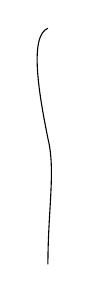
\begin{tikzpicture}\draw (0,0).. controls (-.25,-.1) and (-.1,-.9)..(0,-1.4)..controls (.1,-1.8) and (0,-2.3)..(0,-3);\end{tikzpicture}}
% position: lower prose following table
On \unsure{trouve} que les 2 \unsure{homotopies|contraintes}\deleted{\unsure{compatibilités}} \unsure{comm.}\inserted{sur \(F_{11}\)}
\unsure{sont} \unsure{compatibles}, et \unsure{laissent} une \unsure{indétermination},
qui est un \unsure{hom} de \(M_1\otimes M_2\) en \(L_1\otimes L_2\).
% position: lower isolated formulas
\[
-\qquad E_1\otimes E_2\qquad E_1\otimes E_2
\]
\diagram{$\begin{array}{ll}
\pi'_1=\alpha_1\pi_1\,/\,\omega'_1=\unsure{\varpi_1|\omega_1}\psi_1 & \pi'_1+\bar\omega\\[.6em]
\pi'_2=\alpha_2\pi_2\qquad \unsure{\bar\omega'_2|\varpi'_2}=\omega_2\psi_2 &
\end{array}$}
% position: bottom paragraph
C'est \unsure{normal}, car pour \unsure{l'instant} on n'a \unsure{écrit} \uline{que}
le \unsure{fait} que \unsure{va|on a} \unsure{un} \unsure{iso|de} \unsure{d'extensions|déterminés} - \unsure{et} \unsure{elle}
\unsure{ce|ci} \unsure{sont} \unsure{triviales|faciles}, \unsure{vu|via} \unsure{l'indécision} des choix !
% position: foot pencil
\margin{153}
